% GENERATED by scripts/make_figures.py — do not edit by hand.
% Each caption states the population and block count it draws on,
% so a reader need not infer the statistical scope from Methods.
% Figures are rendered at the exact width declared here; do NOT add
% a scale factor, or the font sizes will no longer be as designed.

\begin{figure}[t]
  \centering
  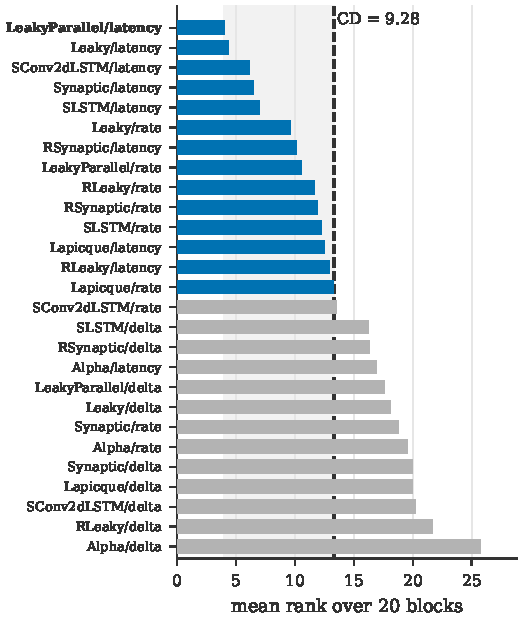
\includegraphics[width=\columnwidth]{figures/fig_screening}
  \caption{Mean macro-F1 rank of all 27 configurations in the \textbf{screening} study, over 20 paired (dataset $\times$ seed) blocks. Friedman $\chi^2=263.9$, $p=3.2e-41$. The shaded band spans one Nemenyi critical difference ($\mathrm{CD}=9.28$) from the leader; the 14 configurations inside it (blue) are not separable from \texttt{LeakyParallel/latency}, which is therefore reported as top-ranked rather than uniquely best.}
  \label{fig:screening}
\end{figure}

\begin{figure*}[t]
  \centering
  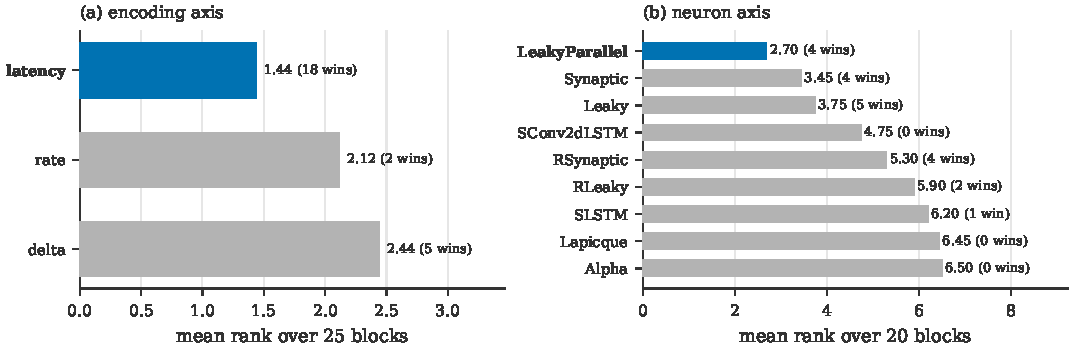
\includegraphics[width=\textwidth]{figures/fig_axes}
  \caption{Strict confirmation along the two design axes. \textbf{(a)} encoding axis: three encodings with the neuron held at \texttt{LeakyParallel}, over 25 paired (protocol $\times$ seed) blocks (Friedman $p=1.5e-03$). \textbf{(b)} neuron axis: nine families with the encoding held at latency, over 20 blocks ($p=1.0e-06$). Bars show mean rank, annotated with blocks won. Each panel holds one factor fixed, so neither --- nor the two together --- reconstructs a strict ranking of all 27 configurations. Note that in (b) the leading family does not win the most individual blocks.}
  \label{fig:axes}
\end{figure*}

\begin{figure*}[t]
  \centering
  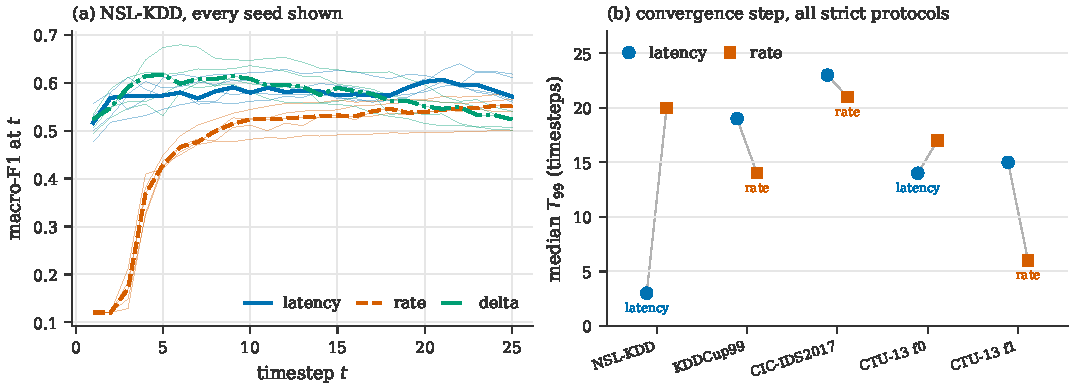
\includegraphics[width=\textwidth]{figures/fig_readout}
  \caption{Temporal evidence accumulation, \texttt{LeakyParallel}, five seeds. \textbf{(a)} macro-F1 as a function of readout step on NSL-KDD; thin lines are individual seeds and thick lines the median, plotted this way because $T_{99}$ is discrete and skewed and a symmetric band would misrepresent it. \textbf{(b)} median $T_{99}$ for latency and rate on all five strict protocols. Latency resolves earlier on two and later on three, so the NSL-KDD advantage (3 against 20 steps) is the strongest case rather than the typical one.}
  \label{fig:readout}
\end{figure*}

\begin{figure}[t]
  \centering
  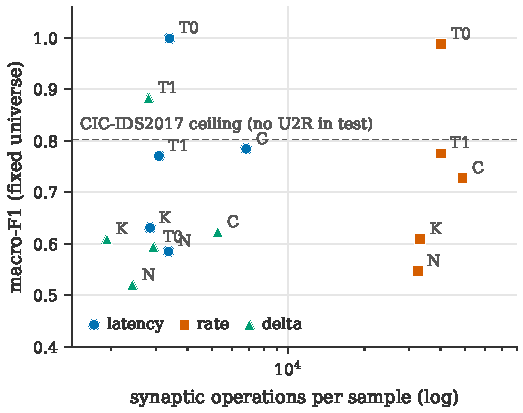
\includegraphics[width=\columnwidth]{figures/fig_pareto}
  \caption{Detection quality against synaptic-operation demand, \texttt{LeakyParallel}, one point per strict protocol and encoding (seed means). Rate encoding requires $7.2\times$ to $13.0\times$ more operations per sample than latency on every protocol, while emitting only $1.7\times$ to $2.5\times$ more spikes in total: the saving comes from where the spikes occur, ahead of the high-fanout input projection, not merely from how many there are. Macro-F1 is the fixed-universe metric, capped at 0.80 on CIC-IDS2017 where U2R has no test support. Point labels give the protocol: N NSL-KDD, K KDDCup99, C CIC-IDS2017, T0/T1 CTU-13 folds.}
  \label{fig:pareto}
\end{figure}

\begin{figure}[t]
  \centering
  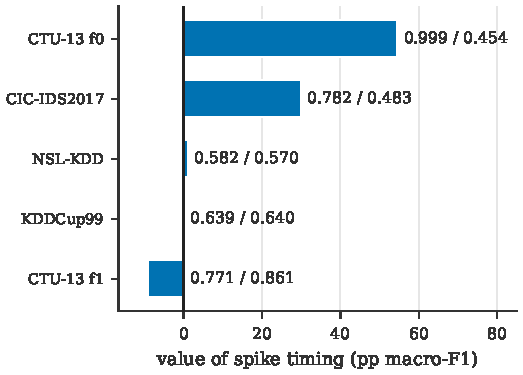
\includegraphics[width=\columnwidth]{figures/fig_timing}
  \caption{\textbf{What spike timing is worth, in isolation.} Each bar is latency coding minus delta coding with both gates set to $\vartheta=0.01$, a construction under which the two arms emit \emph{identical input spike sets} (maximum difference $\FNTimingMaxDiff$ spikes per sample) and differ only in whether the spike carries timing information. Annotations give the two macro-F1 values the difference is taken between, with timing first. LeakyParallel, three seeds, five confirmation protocols. The effect spans $\FNTimingSpread$ percentage points and changes sign, so temporal coding is not a property that helps or hurts in general.}
  \label{fig:timing}
\end{figure}

\begin{figure}[t]
  \centering
  \includegraphics[width=\columnwidth]{figures/fig_sparsitycascade}
  \caption{\textbf{Where latency's efficiency advantage is created and where it is lost.} Ratios of rate to latency on a logarithmic axis, LeakyParallel, five confirmation protocols, five seeds. Input activity separates by $\FNInpRatioMin\times$ to $\FNInpRatioMax\times$, a separation with a closed form that depends on neither dimensionality nor sparsity. Most of it is then diluted: whole-network spike counts differ by only $\FNTotRatioMin\times$ to $\FNTotRatioMax\times$. It reappears in synaptic operations ($\FNSopRatioMin\times$ to $\FNSopRatioMax\times$) because latency's reduction falls ahead of the high-fanout input projection. Where spikes occur matters more than how many there are.}
  \label{fig:sparsitycascade}
\end{figure}

\begin{figure}[t]
  \centering
  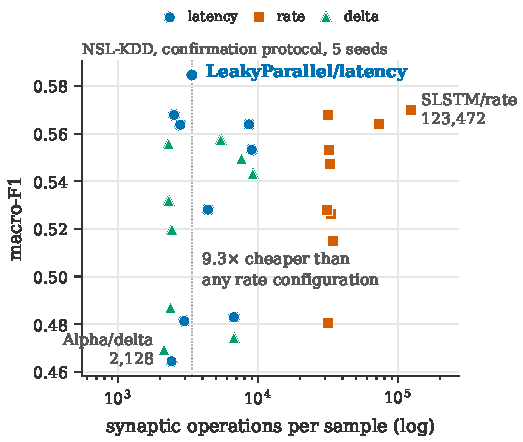
\includegraphics[width=\columnwidth]{figures/fig_pareto27}
  \caption{\textbf{Quality against synaptic operations across the whole design space.} All \FNScrVariants{} configurations on strict NSL-KDD, confirmation protocol, five seeds each, macro-F1 on the fixed label universe. Synaptic operations span 58$\times$ (2,128 to 123,472 per sample) while macro-F1 spans 12.0 percentage points, so most of the design space buys no quality for its cost. \texttt{LeakyParallel/latency} attains the highest macro-F1 of any configuration at 9.3$\times$ fewer operations than the cheapest rate-coded one. No Pareto front is drawn: a staircase here would pass through cheap, weak configurations that are non-dominated only because nothing cheaper exists. Operation counts are not comparable across protocols of differing dimension, so one protocol is shown rather than a pooled average.}
  \label{fig:pareto27}
\end{figure}
